% !TeX root = er.tex

\chapter{Controle}\label{ch.control}

Em robótica, algoritmos tomam decisões. O robô recebe uma tarefa, mas para realizar a tarefa ele deve tomar ações e estas ações dependem do ambiente, conforme detectado pelos sensores. Por exemplo, se um robô deve trazer um objeto de uma prateleira em um armazém para um caminhão de entrega, ele deve usar sensores para navegar até a prateleira apropriada, para detectar e agarrar o objeto, e então navegar de volta para o caminhão e deixar o objeto. Somente robôs que atuam em ambientes extremamente bem definidos podem realizar tais tarefas sem a informação dos sensores. Um exemplo é um braço robótico montando um dispositivo em uma fábrica; se as peças estiverem precisamente posicionadas na superfície de trabalho, o robô pode manipular as peças sem detectá-las. Mas, na maioria dos ambientes, sensores devem ser usados. Em um armazém pode haver obstáculos no caminho até a prateleira, o objeto não será posicionado com precisão na prateleira e o caminhão nunca será estacionado exatamente no mesmo lugar. O robô precisa se adaptar a estas pequenas variações usando \emph{algoritmos de controle} para tomar decisões: com base nos dados dos sensores, que ações o robô precisa realizar para realizar a tarefa? Existe uma sofisticada teoria matemática de controle que é fundamental na robótica. Neste capítulo, apresentamos os conceitos básicos dos algoritmos de controle.

A seção~\ref{s.control-model} explica a diferença entre dois modelos de controle: controle em malha aberta, onde os parâmetros do algoritmo são definidos com antecedência, e controle em malha fechada, onde os dados dos sensores influenciam no comportamento do algoritmo. As seções~\ref{s.on-off}--\ref{s.pid} apresentam quatro algoritmos de controle em malha fechada cada vez mais sofisticados. O projetista de um robô deve escolher entre estes e outros algoritmos similares para selecionar aquele que oferece o desempenho adequado pelo menor custo computacional.

\section{Modelos de Controle}\label{s.control-model}

Há duas maneiras para que um algoritmo decida sobre uma ação. Num sistema em malha aberta, os parâmetros do algoritmo de controle são predefinidos e não mudam enquanto o sistema funciona. Num sistema em malha fechada, os sensores medem o erro entre o estado desejado do sistema e seu estado real, e este erro é usado para decidir que ação tomar.

\subsection{Controle em Malha Aberta}

Uma torradeira é uma máquina que realiza ações semi-autônomas. Você coloca fatias de pão na torradeira, ajusta o temporizador e empurra a alavanca para baixo para iniciar a ação de torrar. Como todos sabemos, os resultados não são garantidos: se a duração do temporizador for muito curta, temos que torrar o pão novamente; se a duração do temporizador for muito longa, o cheiro de torrada queimada flutua através da cozinha. O resultado é incerto porque uma torradeira é um \emph{sistema de controle em malha aberta}. Ele não verifica o resultado da ação do tostador para se certificar que o resultado necessário foi alcançado. Os sistemas em malha aberta são muito familiares: em uma máquina de lavar você pode ajustar a temperatura da água, a duração do ciclo e a quantidade de detergente utilizada, mas a máquina não mede a "limpeza" da roupa (o que quer que isso signifique) e modifica suas ações de maneira correspondente.

Um robô móvel que se desloca para uma posição desejada com base apenas na odometria (Sect.~\ref{s.odometry}) também está utilizando o controle em malha aberta. Ao controlar a potência do motor e a duração do funcionamento dos motores, o robô pode calcular a distância que se moveu. No entanto, variações na velocidade das rodas e na superfície sobre a qual o robô se move causarão incerteza na posição final do robô. Na maioria das aplicações, a odometria pode ser usada para mover o robô para as proximidades da posição desejada, ponto em que são usados outros sensores para mover o robô para a posição desejada exata, por exemplo, usando sensores para medir a distância até um objeto.

\subsection{Controle em Malha Fechada}

Para alcançar um comportamento autônomo, os robôs utilizam \emph{sistemas de controle em malha fechada}. Já encontramos sistemas em malha fechada nos veículos Braintenberg (Activity~\ref{act.attractive}):
\begin{quote}
\normalsize\noindent\textbf{Especificação (Atrativo e repulsivo):} Quando um objeto se aproxima do robô por trás, ele foge até ficar fora de alcance.
\end{quote}
O robô deve \emph{medir} a distância até o objeto e parar quando essa distância for suficientemente grande. O ajuste de potência dos motores depende da medição da distância, mas o robô se move a uma velocidade que depende da potência dos motores, o que muda a distância até o objeto, o que novamente modifica o ajuste de potência, o que faz com que o robô se mova a uma velocidade que depende da potência dos motores, o que muda a distância até o objeto, o que novamente modifica o ajuste de potência, \ldots. Este comportamento circular dá origem ao termo "malha fechada".

Agora formalizamos a especificação de um sistema de controle em malha fechada para um robô (Fig.~\ref{fig.control-model}). A variável $r$ representa o \emph{valor de referencia}, a especificação da tarefa do robô. Para o robô do armazém, os valores de referência incluem a posição do robô em relação a uma pilha de prateleiras e a distância da garra do braço em relação ao objeto a ser pego. Um valor de referência não pode ser usado diretamente pelo robô; ao invés disso, ele deve ser transformado em um \emph{sinal de controle} $u$. Por exemplo, se o valor de referência for a posição do robô em relação a uma prateleira, o sinal de controle será a potência dos motores e a duração que os motores estão em funcionamento. A variável $y$ representa a saída, ou seja, o estado real do robô, por exemplo, a distância até um objeto.

\begin{figure}
\begin{center}
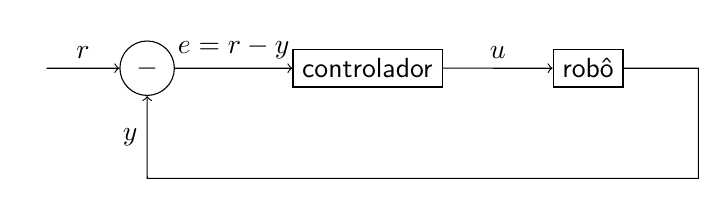
\begin{tikzpicture}[scale=1.4]
\node (input) at (0,1) {};
\node[circle,draw] (diff) at (1,1) {$-$};
\node[rectangle,draw] (control) at (3,1) {\textsf{controlador}};
\node[rectangle,draw] (robot) at (5,1) {\textsf{robô}};
\draw[->] (input) -- node[above] {$r$} (diff);
\draw[->] (diff)  -- node[above] {$e=r-y$} (control);
\draw[->] (control) -- node[above] {$u$} (robot);
\draw[->] (robot) -- ++(1,0) -- ++(0,-1) -- ++(-5,0) -- node[left] {$y$} (diff);
\end{tikzpicture}
\caption{Um sistema de controle em malha fechada}\label{fig.control-model}
\end{center}
\end{figure}

O modelo na Fig.~\ref{fig.control-model} também é chamado de \emph{sistema de controle por realimentação}, porque o valor de saída $y$ é realimentado pelo algoritmo de controle e usado para calcular o sinal de controle. A saída é comparada com o valor de referência para calcular $e=r-y$, o \emph{erro}. O algoritmo de controle usa o valor do erro para gerar o sinal de controle $u$, que é a entrada para o robô.

\subsection{O Período de um Algoritmo de Controle}

Algoritmos de controle são executados periodicamente (Algoritmo~\ref{alg.control-loop}). O software do robô inicializa uma variável \emph{temporizador} que corresponde ao período de execução do algoritmo, por exemplo, a $20$ ms. O computador embarcado tem um \emph{relógio em hardware (clock)} que ``toca'' a intervalos fixos, causando uma interrupção. A interrupção é tratada pelo sistema operacional que decrementa o valor da variável temporizador. Quando o valor desta variável chega a zero, o temporizador expira e um evento é causado em software, levando à execução do algoritmo de controle.

\begin{figure}
\begin{alg}{Esboço do algoritmo de controle}{control-loop}
\hline
&\idv{}integer period&// Duração do período\\
&\idv{}integer timer&// Variável Temporizador\\
\hline
\stl{}&period \ass $\cdots$&// Periodo em milisegundos\\
\stl{}&timer \ass period&// Initializa o temporizador\\
\stl{}&loop&\\
\stl{}&\idc{}when timer-expired-event occurs&\\
\stl{}&\idc{}\idc{}control algorithm&// Executa o algoritmo\\
\stl{}&\idc{}\idc{}timer \ass period&// Reseta o temporizador\\
\hline\hline
&// {\bfseries Sistema Operacional}&\\
\stl{}&when hardware-clock-interrupt occurs&\\
\stl{}&\idc{} timer \ass timer $-$ $1$&// Decrementa o temporizador\\
\stl{}&\idc{} if timer $=$ $0$&// Se temporizador expirou\\
\stl{}&\idc{}\idc{} raise timer-expired-event&// \ \ \ \ causa um evento\\
\end{alg}
\end{figure}

O período de execução do algoritmo é um parâmetro importante no projeto de um sistema de controle. Se o período for muito curto, recursos computacionais valiosos serão desperdiçados e o computador pode ficar sobrecarregado ao ponto de os comandos para o robô chegarem tarde demais. Se o período for muito longo, o robô não responderá a tempo para corrigir erros em seu movimento.

\smallskip

\noindent\textbf{Exemplo} Considere um robô se aproximando a $2$ cm/s de um objeto que está a $10$ cm de distância. Um período de controle de $1$ ms desperdiçaria recursos computacionais porque o robô se moveria apenas $0,002$ cm ($0,02$ mm) durante o ciclo de $1$ ms do algoritmo de controle. Mudanças na potência do motor em distâncias tão pequenas não afetarão a capacidade do robô de cumprir sua tarefa. No extremo oposto, um período de controle de $2$ s é ainda pior: o robô moverá $4$ cm durante este período e provavelmente colidirá com o objeto. Um período de controle de aproximadamente $0,25$ s ($250$ ms) durante o qual o robô se move $0,5$ cm parece um valor razoável para começar, pois $0,5$ cm é uma distância que é significativa em termos de aproximação de um objeto. Você pode experimentar períodos em torno deste valor para determinar o período ideal: um que alcance um comportamento satisfatório com um período o mais longo possível para reduzir o custo computacional.

\begin{framed}
\act{Definição do período de controle}{setperiod}
\begin{itemize}
\item No exemplo anterior, chegamos à conclusão de que o período ótimo do algoritmo de controle foi da ordem de décimos de segundo. Nesta atividade, perguntamos qual deveria ser o período ótimo para outros algoritmos de controle.
\item Um sistema de aquecimento doméstico contém um termostato para controlar a temperatura. Qual seria o período ideal para o algoritmo de controle? O período depende dos parâmetros de engenharia do sistema de aquecimento e das propriedades físicas de como o calor é transferido para as salas. Explique como medir esses fatores e como eles afetam o período de controle.
\item Considere um veículo autônomo tentando estacionar. Que suposições você precisa fazer para definir um período de controle? O que seria um período razoável?
\item Como as propriedades dos sensores afetam o período de controle? Para o exemplo de um robô se aproximando de um objeto, como o período mudaria se o sensor pudesse detectar o objeto a $2$ cm, $5$ cm, $10$ cm, $20$ cm, $40$ cm?
\end{itemize}
\end{framed}

Definimos agora uma sequência de quatro algoritmos de controle, cada um deles baseado no anterior e proporcionando um controle mais preciso, ao preço de uma maior complexidade computacional. Na prática, o projetista do sistema deve escolher o algoritmo mais simples que permita que o robô cumpra sua tarefa.

Os algoritmos são apresentados no contexto de um robô que deve se aproximar de um objeto e parar a uma distância de $s$ em frente a ele. A distância é medida por um sensor de proximidade e a velocidade do robô é controlada através do ajuste da potência dos motores.


\section{Controle Liga-Desliga}\label{s.on-off}


O primeiro algoritmo de controle é chamado de algoritmo \emph{liga-desliga} ou \emph{bang-bang} (Algoritmo~\ref{alg.onoff}). Definimos uma constante \p{referência} que é a distância que o robô deve parar em frente ao objeto. A variável \p{medida} é a distância real medida pelo sensor de proximidade. O \p{erro} é a diferença entre os dois:
\begin{center}
\p{erro} $\leftarrow$ \p{referência} $-$ \p{medida},
\end{center}
que é negativo se o robô estiver muito longe do objeto e positivo se ele estiver muito próximo do objeto. As potências do motor são viradas para frente ou para trás, dependendo do sinal do erro. Por exemplo, se a distância de referência for $10$ cm e a distância medida for $20$ cm, o robô está muito distante e o erro é $10$ cm. Portanto, os motores devem ser ajustados para avançar.
\begin{figure}
\begin{alg}{Controlador Liga-Desliga}{onoff}
&\idv{}integer reference \ass $\cdots$&// Distância de referência\\
&\idv{}integer measured &// Distância medida\\
&\idv{}integer error &// Erro de distância\\
\hline
\stl{}&error \ass reference $-$ measured&\\
\stl{}&if error $<$ 0&\\
\stl{}&\idc{} left-motor-power \ass $100$&// Move para frente\\
\stl{}&\idc{} right-motor-power \ass $100$&\\
\stl{}&if error $=$ 0&\\
\stl{}&\idc{} left-motor-power \ass $0$&// Desliga motores\\
\stl{}&\idc{} right-motor-power \ass $0$&\\
\stl{}&if error $>$ 0&\\
\stl{}&\idc{} left-motor-power \ass $-100$&// Move para trás\\
\stl{}&\idc{} right-motor-power \ass $-100$&\\
\end{alg}
\end{figure}

O robô se aproxima do objeto em velocidade máxima. Quando o robô atinge a distância de referência do objeto, leva tempo para que o sensor seja lido e o erro seja computado. Mesmo que o robô meça uma distância exatamente igual à distância de referência (o que é improvável), o robô não será capaz de parar imediatamente e irá ultrapassar a distância de referência. O algoritmo então fará com que o robô se mova para trás à velocidade máxima, passando novamente a distância de referência. Quando o temporizador faz com que o algoritmo de controle seja executado novamente, o robô inverterá a direção novamente e seguirá para frente a toda velocidade. O comportamento resultante do robô é mostrado na Fig.~\ref{fig.onoff}: o robô irá oscilar em torno da distância de referência ao objeto. É altamente improvável que o robô realmente pare na distância de referência ou próximo a ela.

\begin{figure}
\begin{center}
\begin{tikzpicture}[scale=1.2]
\draw[<->] (0,5) -- node[sloped,above,rotate=180] {\p{distance}} (0,0) node[left] {} -- node[below] {\p{time}} (8,0);
\draw (0,2) node[below right] {$r$} -- (8,2);
\draw[thick] plot coordinates {(0,5) (2,1.5) (3,2.5) (4,1.5) (5,2.5) (6,1.5)(7,2.5) (8,1.5)};
\end{tikzpicture}
\caption{Comportamento do algoritmo Liga-Desliga}\label{fig.onoff}
\end{center}
\end{figure}

Uma desvantagem adicional do algoritmo liga-desliga é que a inversão de direção frequente e abrupta resulta em altas acelerações. Se estivermos tentando controlar um braço com garra, os objetos que ele está carregando podem ser danificados. O algoritmo também gera altos níveis de desgaste nos motores e em outras partes móveis mecânicas.

\begin{framed}
\act{Controlador Liga-Desliga}{onoff}
\begin{itemize}
\item Implemente o algoritmo liga-desliga para seu robô executar a tarefa de parar a uma distância de referência de um objeto.
\item Execute-o várias vezes a partir de distâncias diferentes do objeto.
\item O Algoritmo \ref{alg.onoff} pára o robô quando o erro é exatamente zero. Modifique a implementação para que o robô pare se o erro estiver dentro de uma pequena distância em torno de zero. Experimente com faixas diferentes e veja como elas afetam o comportamento do robô.
\end{itemize}
\end{framed}

\section{Controlador proporcional (P)}\label{s.p}

Para desenvolver um algoritmo melhor, nos inspiramos em andar de bicicleta. Suponha que você esteja andando de bicicleta e veja que o semáforo à sua frente ficou vermelho. Você não espera até o último momento quando estiver na linha de parada para apertar com força máxima a alavanca do freio. Se fizer isso, você pode ser atirado da bicicleta! O que você faz é diminuir sua velocidade gradualmente: primeiro, você pára de pedalar; depois, você aperta o freio suavemente para diminuir um pouco mais a velocidade; finalmente, quando você está na linha de parada e vai devagar, você aperta com mais força para parar completamente a bicicleta. O algoritmo usado por um ciclista pode ser expresso como:
\begin{quote}
\normalsize\noindent{}Reduza mais sua velocidade à medida que você se aproxima da distância de referência.
\end{quote}
A diminuição da velocidade é (inversamente) \emph{proporcional} ao quão próximo você está do semáforo: quanto mais próximo você está, mais você freia. O fator de proporcionalidade é chamado de \emph{ganho} do algoritmo de controle. Uma maneira alternativa de expressar este algoritmo é:
\begin{quote}
\normalsize\noindent{}Reduza mais sua velocidade à medida que o erro entre a distância de referência e a distância medida fica menor.
\end{quote}

Algoritmo~\ref{alg.proportional} é o \emph{algoritmo de controle proporcional} ou um \emph{Controlador P}.

\begin{figure}
\begin{alg}{Controlador Proporcional}{proportional}
&\idv{}integer reference \ass $\cdots$&// Distância de Referência\\
&\idv{}integer measured &// Distância Medida\\
&\idv{}integer error &// Erro\\
&\idv{}float gain \ass $\cdots$& // Ganho Proporcional\\
&\idv{}integer power & // Potência do Motor\\
\hline
\stl{}&error \ass reference $-$ measured&// Distâncias\\
\stl{}&power \ass gain * error&// Sinal de Controle\\
\stl{}&left-motor-power \ass power&\\
\stl{}&right-motor-power \ass power&\\
\end{alg}
\end{figure}

\smallskip

\noindent\textbf{Exemplo} Suponha que a distância de referência seja de $100$ cm e o ganho seja $-0,8$. Quando o robô está a $150$ cm do objeto, o erro é $100-150=-50$ e o algoritmo de controle ajustará a potência para $-0,8\cdot -50=40$. A tabela~\ref{tab.p-controller} mostra os erros e as configurações de potência para três distâncias. Se o robô ultrapassar a distância de referência de $100$ cm e uma distância de $60$ cm for medida, a potência será ajustada para $-32$ fazendo com que o robô se mova para trás.

\begin{table}
\caption{Controlador proporcional com ganho de $-0,8$}
\label{tab.p-controller}
\begin{tabular}{rrr}
\hline\noalign{\smallskip}
\multicolumn{1}{c}{Distância} & \multicolumn{1}{c}{\ \ \ Erro}& \multicolumn{1}{c}{\ \ \ Potência}\\
\noalign{\smallskip}\hline\noalign{\smallskip}
$150$ & $-50$ & $40$\\
$125$ & $-25$ & $20$\\
$60$ & $40$ & $-32$\\
\noalign{\smallskip}\hline\noalign{\smallskip}
\end{tabular}
\end{table}

A Figura~\ref{fig.p-control} traça a distância do robô ao objeto como uma função do tempo quando o robô é controlado por um controlador P. A linha $r$ indica a distância de referência. A mudança na potência do motor é suave para que o robô não experimente acelerações e desacelerações muito elevadas. A resposta é um pouco lenta, mas o robô se aproxima da distância de referência.

\begin{figure}
\begin{center}
\begin{tikzpicture}[scale=1.2]
\draw[<->] (0,5) -- node[sloped,above,rotate=180] {\p{distância}} (0,0) node[left] {} -- node[below] {\p{tempo}} (8,0);
\draw (0,1.9) node[below right] {$r$} -- (8,1.9);
\draw[domain=0:8,samples=100,thick] plot (\x,{3*exp(-2*\x)+2});
\end{tikzpicture}
\caption{Comportamento do controlador P}\label{fig.p-control}
\end{center}
\end{figure}

Infelizmente, o robô não atinge realmente a distância de referência. Para entender o porquê, considere o que acontece quando o robô está muito próximo da distância de referência. O erro será muito pequeno e, consequentemente, a potência será muito baixa. Em teoria, o ajuste de baixa potência deve fazer com que o robô se mova lentamente, alcançando a distância de referência em algum momento. Na prática, a potência do motor pode se tornar tão baixa que não será capaz de superar o atrito interno nos motores e sua conexão com as rodas, de modo que o robô pare de se mover.

Pode parecer que aumentar o ganho do controlador P poderia superar este problema, mas um ganho alto sofre de uma séria desvantagem. A figura~\ref{fig.gain} mostra o efeito do ganho no controlador P. Um ganho maior (linha vermelha tracejada) faz com que o robô se aproxime mais rapidamente da distância de referência, enquanto um ganho menor (linha azul tracejada) faz com que o robô se aproxime mais lentamente. Entretanto, se o ganho for muito alto, o controlador P funciona como um controlador liga-desliga com uma resposta oscilante (linha verde). Dizemos que o controlador é \emph{oscilatório}\footnote{N. do T.: O texto original usa o termo "unstable", mas nós preferimos não utilizar a tradução "instável" pois, de acordo com a definição de estabilidade encontrada na literatura de controle em lígua portuguesa, o sinal mostrado refere-se a um sistema (marginalmente) estável, ainda que oscilatório, pois tem saída limitada para entrada limitada.}.


\begin{figure}
\begin{center}
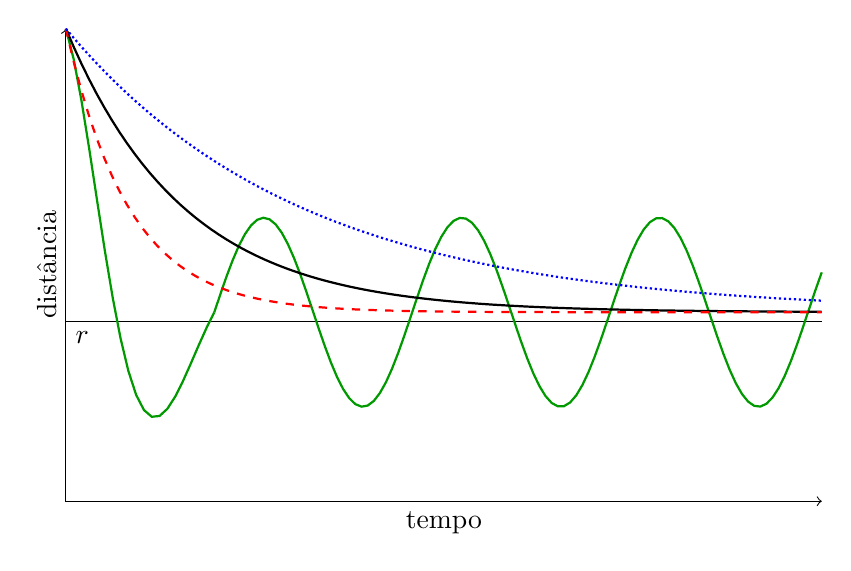
\begin{tikzpicture}[scale=1.2]
\draw[<->] (0,5) -- node[sloped,above,rotate=180] {\p{distância}} (0,0) node[left] {} -- node[below] {\p{tempo}} (8,0);
\draw (0,1.9) node[below right] {$r$} -- (8,1.9);
\draw[domain=0:1.57,samples=20,thick,green!60!black] plot (\x,{3*exp(-\x)*cos(3*\x r)+2});
\draw[domain=1.57:8,samples=100,thick,green!60!black] plot (\x,{cos(3*\x r)+2});
\draw[domain=0:8,samples=100,thick] plot (\x,{3*exp(-.8*\x)+2});
\draw[domain=0:8,samples=100,dashed,red,thick] plot (\x,{3*exp(-1.5*\x)+2});
\draw[domain=0:8,samples=100,densely dotted,blue,thick] plot (\x,{3*exp(-.4*\x)+2});
\end{tikzpicture}
\caption{O efeito do ganho no controlador P: ganho menor (linha azul tracejada), ganho maior (linha vermelha tracejada), ganho excessivo (linha verde)}\label{fig.gain}
\end{center}
\end{figure}

Há situações em que o controlador P não pode alcançar a distância de referência mesmo em um sistema ideal. Suponha que o objeto em si esteja se movendo a uma velocidade constante para longe do robô. O controlador P ajustará a potência máxima do motor para fazer com que o robô se mova rapidamente em direção ao objeto. Eventualmente, porém, conforme o robô se aproxima do objeto, a distância medida se tornará pequena e o controlador P definirá a potência tão baixa que a velocidade do robô será menor que a velocidade do objeto. O resultado é que o robô nunca alcançará a distância de referência. Se o robô pudesse realmente alcançar a distância de referência, o erro seria zero e, portanto, a velocidade do robô também seria zero. O objeto, entretanto, ainda está se afastando do robô, então um pouco mais tarde o robô começará a se mover novamente e o ciclo se repete. Este movimento de partida e parada não é o objetivo pretendido de manter a distância de referência.

\smallskip

\noindent\textbf{Exemplo} Utilizamos os mesmos dados do exemplo anterior, exceto que o objeto se move a $20$ cm/s. A tabela~\ref{tab.p-controller-moving} mostra os erros e as potências resultantes para cada caso. Inicialmente, o robô está indo mais rápido do que o objeto, então ele o alcançará. A $125$ cm do objeto, entretanto, o robô está se movendo na mesma velocidade que o objeto. Ele mantém esta distância fixa e não se aproximará da distância de referência de $100$ cm. Se de alguma forma o robô se aproximar do objeto, digamos, $110$ cm, a potência é reduzida para $8$ fazendo com que o robô se afaste do objeto.

\begin{table}
\caption{Controlador proporcional para um objeto em movimento e um ganho de $-0,8$}
\label{tab.p-controller-moving}
\begin{tabular}{rrr}
\hline\noalign{\smallskip}
\multicolumn{1}{c}{distância} & \multicolumn{1}{c}{\ \ \ erro}& \multicolumn{1}{c}{\ \ \ potência}\\
\noalign{\smallskip}\hline\noalign{\smallskip}
$150$ & $-50$ & $40$\\
$125$ & $-25$ & $20$\\
$110$ & $-10$ & $8$\\
\noalign{\smallskip}\hline\noalign{\smallskip}
\end{tabular}
\end{table}

Em geral, o robô se estabilizará a uma distância fixa da distância de referência. Você pode reduzir este erro aumentando o ganho, mas a distância de referência nunca será alcançada e o único resultado é que o controlador se torna instável.

\begin{framed}
\act{Controlador Proporcional}{proportional}
\begin{itemize}
\item Implemente o algoritmo de controle proporcional para fazer o robô parar a uma distância especificada de um objeto. Com que precisão você pode alcançar o objetivo quando o objeto não se move?
\item O que acontece se o objeto se move? Para o objeto, você pode usar um segundo robô programado para se mover a uma velocidade fixa.
\item Experimente com o ganho e o período para ver como eles afetam o desempenho do algoritmo.
\end{itemize}
\end{framed}

\section{Controlador Proporcional-Integral (PI)}\label{s.pi}

Um \emph{controlador proporcional-integral} pode alcançar a distância de referência mesmo na presença de atrito ou um objeto em movimento levando em conta o erro acumulado ao longo do tempo. Enquanto o controlador P leva em conta apenas o erro atual
\[
u(t) = k_pe(t)\,,
\]
o controlador PI adiciona a integral do erro desde o momento em que o algoritmo começa a funcionar até o presente momento:
\[
u(t) = k_pe(t) + k_i\int_{0}^t e(\tau)\,d\tau\,.
\]
Diferentes valores de ganho são usados para os termos proporcional e integral para permitir flexibilidade no projeto do controlador.

Para programar um controlador PI, uma aproximação discreta da integral contínua é realizada (Algorithm~\ref{alg.pi-controller}).

\begin{figure}
\begin{alg}{Controlador Proporcional-Integral}{pi-controller}
&\idv{}integer reference \ass $\cdots$&// Distância de referência\\
&\idv{}integer measured &// Distância medida\\
&\idv{}integer error &// Erro\\
&\idv{}integer error-sum $\leftarrow 0$&// Erro acumulado\\
&\idv{}float gain-p \ass $\cdots$& // Ganho proporcional\\
&\idv{}float gain-i \ass $\cdots$& // Ganho integral\\
&\idv{}integer power & // Potência do motor\\
\hline
\stl{}&error \ass reference $-$ measured&// Distâncias\\
\stl{}&error-sum \ass error-sum + error&// Termo integral\\
\stl{}&power \ass gain-p * error + gain-i * error-sum&// Sinal de controle\\ 
\stl{}&left-motor-power \ass power&\\
\stl{}&right-motor-power \ass power&\\
\end{alg}
\end{figure}

Na presença de atrito ou de um objeto em movimento, o erro será integrado (acumulado) e fará com que a potência do motor seja maior; isto fará com que o robô converja para a distância de referência. Um problema com um controlador PI é que a integração do erro parte do estado inicial quando o robô está longe do objeto. Conforme o robô se aproxima da distância de referência, o termo integral do controlador já terá um grande valor; para diminuir este valor, o robô deve ultrapassar a distância de referência para que haja erros de sinal oposto. Isto pode gerar oscilações (Fig.~\ref{fig.pi-control}).

\begin{figure}
\begin{center}
\begin{tikzpicture}[scale=1.2]
\draw[<->] (0,5) -- node[sloped,above,rotate=180] {\p{distância}} (0,0) node[left] {} -- node[below] {\p{tempo}} (8,0);
\draw (0,2) node[below right,xshift=-1pt] {$r$} -- (8,2);
\draw[domain=0:8,samples=100,thick] plot (\x,{3*exp(-1*\x)*cos(5*\x r)+2});
\end{tikzpicture}
\caption{Comportamento do controlador PI}\label{fig.pi-control}
\end{center}
\end{figure}

\begin{framed}
\act{Controlador PI}{PIcontroller}
\begin{itemize}
\item Implemente um controlador PI que faça o robô parar a uma distância especificada de um objeto.
\item Compare o comportamento do controlador PI com um controlador P para a mesma tarefa, monitorando as variáveis dos algoritmos de controle ao longo do tempo.
\item O que acontece se você manualmente impedir o robô de se mover por um curto período de tempo e depois deixá-lo ir? Isto demonstra um conceito chamado em inglês de \emph{windup}\footnote{N. do T.: Preferimos manter o termo "windup" em inglês pois ele é amplamente utilizado na literatura de controle em língua portuguesa.}. Explore o conceito através de fontes online e encontre um método para corrigir esse problema.
\end{itemize}
\end{framed}

\section{Controlador Proporcional-Integral-Derivativo (PID)}\label{s.pid}

Quando você lança ou chuta uma bola para outro jogador que está se movendo, você não a lança para a posição atual do jogador. Caso contrário, ele já terá se movido para uma nova posição quando a bola chegar. Ao invés disso, você estima sua futura posição e lança a bola para lá. Da mesma forma, um robô cuja tarefa é empurrar um pacote para um carrinho em movimento deve cronometrar seu empurrão para a posição futura estimada do carrinho quando o pacote chegar a ele. O algoritmo de controle deste robô não pode ser um controlador liga-desliga, P ou PI, porque eles só levam em conta o valor atual do erro (e os valores anteriores no caso do controlador PI). 

Para estimar o erro futuro, a taxa de mudança do erro deve ser levada em conta. Se a taxa de mudança do erro for pequena, o robô pode empurrar o pacote imediatamente antes da aproximação do carrinho, enquanto que se a taxa de mudança do erro for grande, o pacote deve ser empurrado muito mais cedo.

Matematicamente, a taxa de mudança é expressa como uma derivada. Um controlador \emph{Proporcional-Integral-Derivativo (PID)} acrescenta um termo adicional aos termos P e I:
\begin{equation}
u(t) = k_pe(t) + k_i\int_{\tau=0}^t e(\tau)\,d\tau + k_d \frac{de(t)}{dt}\,.\label{eq.pid}
\end{equation}

Na implementação de um controlador PID, o diferencial é aproximado pela diferença entre o erro anterior e o erro atual (Algorithm~\ref{alg.pid-controller}).

\begin{figure}
\begin{alg}{Controlador Proporcional-Integral-Derivativo}{pid-controller}
&\idv{}integer reference \ass $\cdots$&// Distância de referência\\
&\idv{}integer measured &// Distância medida\\
&\idv{}integer error &// Erro\\
&\idv{}integer error-sum $\leftarrow 0$ &// Erro acumulado\\
&\idv{}integer previous-error \ass 0&// Erro anterior\\
&\idv{}integer error-diff &// Diferença de erro\\
&\idv{}float gain-p \ass $\cdots$& // Ganho proporcional\\
&\idv{}float gain-i \ass $\cdots$& // Ganho integral\\
&\idv{}float gain-d \ass $\cdots$& // Ganho derivativo\\
&\idv{}integer power & // Poência do motor\\
\hline
\stl{}&error \ass reference $-$ measured&// Distâncias\\
\stl{}&error-sum \ass error-sum + error&// Termo integral\\
\stl{}&error-diff \ass error $-$ previous-error&// Termo differencial\\
\stl{}&previous-error \ass error&// Salva erro atual\\
\stl{}&power \ass gain-p * error + &// Sinal de controle\\ 
&\idc{}gain-i * error-sum + gain-d * error-diff&\\ 
\stl{}&left-motor-power \ass power&\\
\stl{}&right-motor-power \ass power&\\
\end{alg}
\end{figure}

O comportamento do controlador PID é mostrado na Fig.~\ref{fig.pid-control}. O robô converge de forma suave e rápida para a distância de referência. 

\begin{figure}
\begin{center}
\begin{tikzpicture}[scale=1.2]
\draw[<->] (0,5) -- node[sloped,above,rotate=180] {\p{distância}} (0,0) node[left] {} -- node[below] {\p{tempo}} (8,0);
\draw[dashed] (0,2) node[below right] {$r$} -- (8,2);
\draw[domain=0:8,samples=100,thick] plot (\x,{2.5*exp(-2*\x)+2});
\end{tikzpicture}
\caption{Comportamento do controlador PID}\label{fig.pid-control}
\end{center}
\end{figure}

Os ganhos de um controlador PID devem ser cuidadosamente ajustados. Se os ganhos para os termos P e I forem muito altos, podem ocorrer oscilações. Se o ganho para o termo D for muito alto, o controlador reagirá a pequenos picos de ruído.

\begin{framed}
\act{Controlador PID}{PIDcontroller}
\begin{itemize}
\item Implemente um controlador PID para a tarefa de um robô que se aproxima de um objeto.
\item Experimente com diferentes ganhos até que o robô se aproxime suavemente da distância de referência.
\item Repita os experimentos com um objeto em movimento.
\end{itemize}
\end{framed}

\section{Sumário}

Um bom algoritmo de controle deve convergir rapidamente para o resultado desejado enquanto
evita movimentos bruscos. Deve ser computacionalmente eficiente e não deve requerer ajustes constantes. O algoritmo de controle tem de ser adaptado às exigências específicas do sistema e da tarefa, e funcionar corretamente em diferentes condições ambientais. Descrevemos quatro algoritmos, desde o impraticável algoritmo liga-desliga até algoritmos que combinam termos proporcional, integral e derivativo. O termo proporcional garante que grandes erros causem rápida convergência para a referência, o termo integral garante que a referência possa ser realmente alcançada, enquanto o termo derivativo torna o algoritmo mais responsivo. 

\section{Leitura adicional}

Um moderno livro didático sobre algoritmos de controle é \cite{astrom-murray}.
